\begin{usecase}{View Integrated Calendar}
  \ucbasicinfo{High}{Regular}
  \ucshortdescription{Allows users to view their calendar events using iOS EventKit integration}
  \uctrigger{User opens the calendar view in the app.}
  \ucactors{User}{EventKit}
  \ucpreconditions{
    \begin{itemize}
      \item User must be logged in
      \item Calendar access must be authorized in iOS Settings
    \end{itemize}
  }
  \ucrelationships{N/A}{N/A}{N/A}
  \ucinputsoutputs{
    \begin{itemize}
      \item \textbf{Calendar data} (Source: EventKit)
      \item \textbf{View preferences} (Source: User settings)
    \end{itemize}
  }{
    \begin{itemize}
      \item \textbf{Integrated calendar view} (Destination: App UI)
    \end{itemize}
  }
  \ucmainflow{
    \begin{enumerate}
      \item The user opens the calendar view.
            \ucinfo{The app queries EventKit for calendars and events.}
      \item EventKit provides calendar and event data.
            \ucinfo{The app processes and displays events.}
      \item The app updates in real-time as EventKit receives changes.
            \ucinfo{Changes from the Baikal server or other sources are reflected immediately when EventKit notifies us.}
    \end{enumerate}
  }
  \ucconclusion{User views their calendar events in a unified interface powered by EventKit.}
  \ucpostconditions{Calendar events are displayed and stay in sync with iOS Calendar.}
  \ucspecialrequirements{
    \begin{itemize}
      \item The app must observe EventKit changes for real-time updates.
      \item The app must handle calendar access permissions gracefully.
    \end{itemize}
  }
  \ucbusinessrules{
    \begin{itemize}
      \item \textbf{Events must be displayed according to user preferences.}
      \item \textbf{All calendar sources must be treated equally in the integrated view.}
    \end{itemize}
  }
\end{usecase}

\begin{figure}[!h]
  \centering
  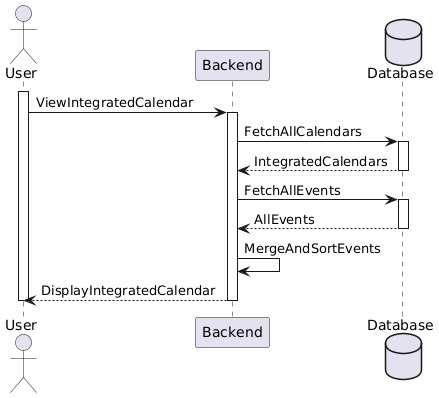
\includegraphics[width=0.6\textwidth]{images/docs/diagrams/sequence-diagrams/all-sequence-diagrams/View Integrated Calendar.png}
  \caption{View Integrated Calendar Sequence Diagram}
  \label{fig:seq/view-integrated-calendar}
\end{figure}

The ``View Integrated Calendar Sequence Diagram'', shown in \textbf{Figure~\ref{fig:seq/view-integrated-calendar}}, demonstrates how the app leverages iOS EventKit to provide a unified calendar view. The sequence begins when the user opens the calendar view in the app.

The app uses EventKit to access calendar and event data directly from iOS's calendar database. This includes events from our Baikal server (synced via CalDAV) and any other calendars the user has configured. EventKit provides real-time updates through its observer system, ensuring the app's display stays synchronized with the system calendar.

This client-side approach eliminates the need for separate backend queries, as EventKit efficiently manages data access and synchronization. The app focuses on presenting the data in a user-friendly way, applying custom styling and organization while maintaining consistency with the iOS Calendar app.